%% LaTeX-Abbildungsdefinitionen mit TikZ
%% Verwendet in den Kapiteln über \ref{fig:...}

\tikzset{
  block/.style={rectangle, draw, fill=blue!20, text width=2.5cm, text centered, rounded corners, minimum height=1cm},
  db/.style={cylinder, draw, fill=green!20, text width=2.5cm, text centered, minimum height=1cm},
  externa/.style={rectangle, draw, fill=gray!20, text width=2.5cm, text centered, rounded corners, minimum height=0.8cm},
  arrow/.style={->, thick, >=stealth},
}

%% DIAGRAM 1: System Architecture (3-Schichten + Externe)
\newcommand{\DiagramSystemArchitektur}{%
\begin{tikzpicture}[node distance=1.6cm, auto]

  % External Services
  \node[externa] (fapi) at (0, 2.4)  {Football-API\\api-sports.io};
  \node[externa] (llm)  at (0, 0.4)  {LLM Provider\\OpenRouter};
  \node[externa] (sp)   at (0, -1.6) {ScorePlay\\Media};

  % Integrationsschicht
  \node[block] (n8n) at (4, 0.4) {n8n\\Workflows};

  % Anwendungsschicht
  \node[block] (api) at (8, 1.4)  {FastAPI\\Backend};
  \node[db]    (db)  at (8, -0.8) {PostgreSQL};

  % Präsentationsschicht
  \node[block] (fe) at (12, 0.4) {React\\Frontend};

  % Layer background boxes
  \begin{pgfonlayer}{background}
    \node[draw=gray!50, fill=gray!8, rounded corners=4pt, inner sep=8pt,
          fit=(fapi)(llm)(sp)] (ext_box) {};
    \node[draw=blue!35, fill=blue!4, rounded corners=4pt, inner sep=10pt,
          fit=(n8n)] (int_box) {};
    \node[draw=blue!35, fill=blue!4, rounded corners=4pt, inner sep=10pt,
          fit=(api)(db)] (app_box) {};
    \node[draw=blue!35, fill=blue!4, rounded corners=4pt, inner sep=10pt,
          fit=(fe)] (pres_box) {};
  \end{pgfonlayer}

  % Arrows
  \draw[arrow] (fapi) -- (n8n);
  \draw[arrow] (sp)   -- (n8n);
  \draw[arrow] (llm)  -- (n8n);
  \draw[arrow] (llm.north) to[out=80, in=155] (api.north west);
  \draw[arrow] (n8n)  -- (api);
  \draw[arrow] (n8n)  -- (db);
  \draw[arrow] (api)  -- (db);
  \draw[arrow] (api)  -- (fe);
  \draw[arrow] (fe)   -- (api);
  \draw[arrow] (fe.north) to[out=130, in=50, looseness=0.55]
    node[above, font=\scriptsize] {Webhook-Trigger} (n8n.north);

  % Layer labels below boxes
  \node[below=0.25cm of ext_box,  font=\small\itshape] {Externe Dienste};
  \node[below=0.25cm of int_box,  font=\small\itshape] {Integrationsschicht};
  \node[below=0.25cm of app_box,  font=\small\itshape] {Anwendungsschicht};
  \node[below=0.25cm of pres_box, font=\small\itshape] {Präsentationsschicht};

\end{tikzpicture}%
}


%% DIAGRAM 3: Ticker State Transitions
\newcommand{\DiagramTickerStates}{%
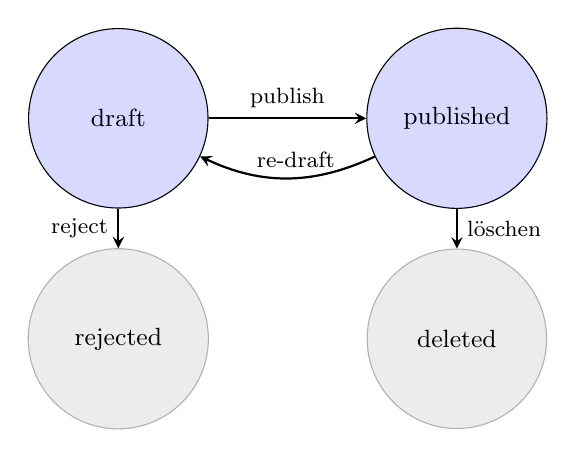
\begin{tikzpicture}[node distance=2.8cm, auto]
  \tikzset{
    active/.style={circle, draw, fill=blue!15, text width=2.0cm,
                   text centered, minimum size=2.2cm, font=\small},
    terminal/.style={circle, draw=gray!60, fill=gray!15, text width=2.0cm,
                     text centered, minimum size=2.2cm, font=\small},
  }

  % Active states (top row)
  \node[active] (draft)     {draft};
  \node[active, right of=draft, xshift=1.5cm] (published) {published};

  % Terminal states (bottom row)
  \node[terminal, below of=draft]     (rejected) {rejected};
  \node[terminal, below of=published] (deleted)  {deleted};

  % Transitions — no crossing arrows
  \draw[arrow] (draft)     -- node[above]{\footnotesize publish}   (published);
  \draw[arrow] (draft)     -- node[left] {\footnotesize reject}    (rejected);
  \draw[arrow] (published) -- node[right]{\footnotesize löschen}   (deleted);
  \draw[arrow, bend left=25] (published) to
        node[above, pos=0.45]{\footnotesize re-draft} (draft);
\end{tikzpicture}%
}


%% DIAGRAM 5: Logical Data Model (simplified ER)
\newcommand{\DiagramDataModel}{%
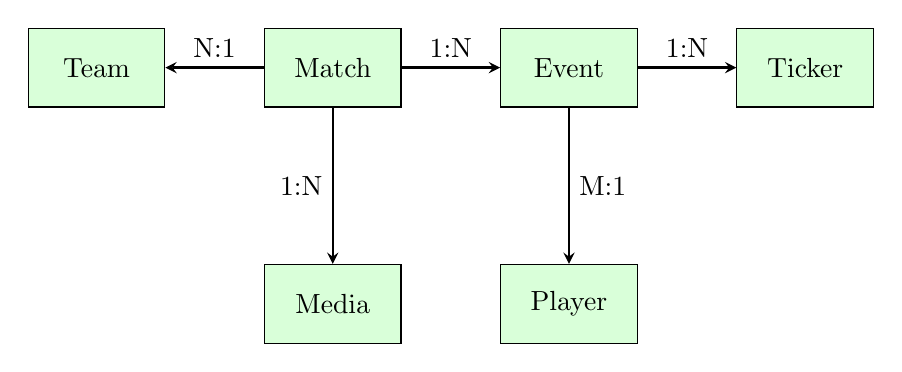
\begin{tikzpicture}[node distance=3cm, auto]
  \tikzset{entity/.style={rectangle, draw, fill=green!15, text width=1.5cm, text centered, minimum height=1cm}}

  \node[entity] (team)   {Team};
  \node[entity, right of=team]  (match)  {Match};
  \node[entity, right of=match] (event)  {Event};
  \node[entity, right of=event] (ticker) {Ticker};
  \node[entity, below of=match] (media)  {Media};
  \node[entity, below of=event] (player) {Player};

  \draw[arrow] (match)  -- node[above] {N:1} (team);
  \draw[arrow] (match)  -- node[above] {1:N} (event);
  \draw[arrow] (event)  -- node[above] {1:N} (ticker);
  \draw[arrow] (match)  -- node[left]  {1:N} (media);
  \draw[arrow] (event)  -- node[right] {M:1} (player);
\end{tikzpicture}%
}

%% DIAGRAM 6: Communication Flow
\newcommand{\DiagramCommunicationFlow}{%
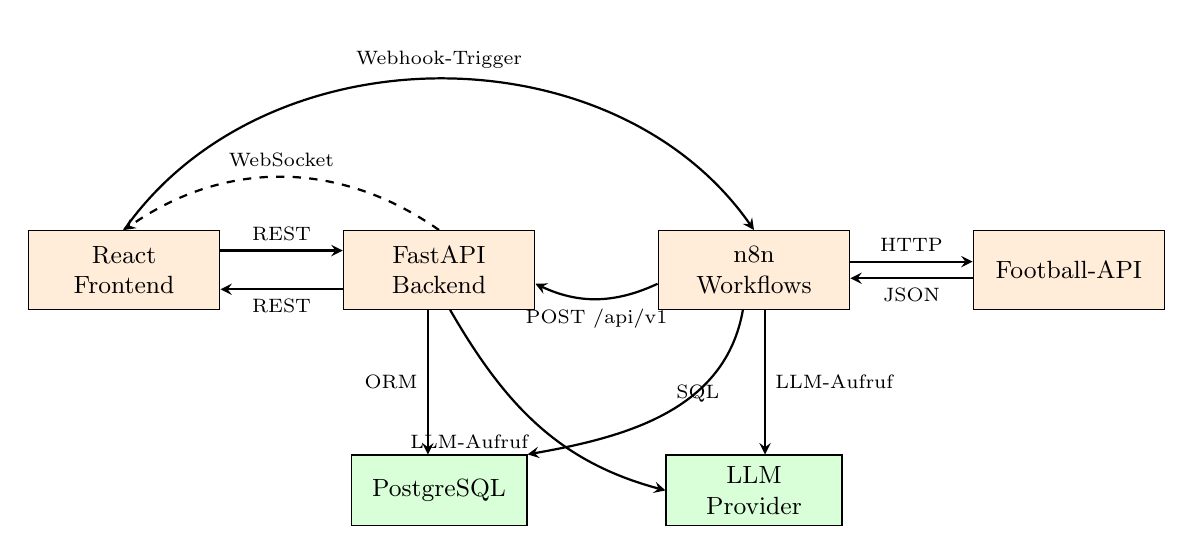
\begin{tikzpicture}[auto]
  \tikzset{
    actor/.style={rectangle, draw, fill=orange!15, text width=2.2cm,
      text centered, minimum height=1cm, font=\small},
    store/.style={rectangle, draw, fill=green!15, text width=2.0cm,
      text centered, minimum height=0.9cm, font=\small},
  }

  % Obere Reihe: Laufzeitkomponenten
  \node[actor] (fe)  at (0,  0) {React\\Frontend};
  \node[actor] (be)  at (4,  0) {FastAPI\\Backend};
  \node[actor] (n8n) at (8,  0) {n8n\\Workflows};
  \node[actor] (api) at (12, 0) {Football-API};

  % Untere Reihe: Datenhaltung und KI
  \node[store] (db)  at (4,  -2.8) {PostgreSQL};
  \node[store] (llm) at (8,  -2.8) {LLM\\Provider};

  % Frontend ↔ Backend (REST)
  \draw[arrow] ([yshift= 7pt]fe.east) -- node[above, font=\scriptsize] {REST}
               ([yshift= 7pt]be.west);
  \draw[arrow] ([yshift=-7pt]be.west) -- node[below, font=\scriptsize] {REST}
               ([yshift=-7pt]fe.east);

  % Backend → Frontend (WebSocket, gestrichelt)
  \draw[arrow, dashed] (be.north) to[out=145, in=35]
    node[above, font=\scriptsize] {WebSocket} (fe.north);

  % Frontend → n8n (Webhook-Trigger)
  \draw[arrow] (fe.north) to[out=55, in=125]
    node[above, font=\scriptsize] {Webhook-Trigger} (n8n.north);

  % n8n → Backend (POST)
  \draw[arrow] ([yshift=-5pt]n8n.west) to[out=205, in=335]
    node[below, font=\scriptsize] {POST /api/v1} ([yshift=-5pt]be.east);

  % n8n ↔ Football-API
  \draw[arrow] ([yshift= 3pt]n8n.east) -- node[above, font=\scriptsize] {HTTP}
               ([yshift= 3pt]api.west);
  \draw[arrow] ([yshift=-3pt]api.west) -- node[below, font=\scriptsize] {JSON}
               ([yshift=-3pt]n8n.east);

  % Backend → PostgreSQL (ORM, vertikal)
  \draw[arrow] ([xshift=-4pt]be.south) -- node[left, font=\scriptsize] {ORM}
               ([xshift=-4pt]db.north);

  % Backend → LLM Provider
  \draw[arrow] ([xshift=4pt]be.south) to[out=300, in=165]
    node[below left, font=\scriptsize] {LLM-Aufruf} (llm.west);

  % n8n → PostgreSQL (direktes SQL)
  \draw[arrow] ([xshift=-4pt]n8n.south) to[out=260, in=10]
    node[above right, font=\scriptsize] {SQL} (db.north east);

  % n8n → LLM Provider (vertikal)
  \draw[arrow] ([xshift=4pt]n8n.south) -- node[right, font=\scriptsize] {LLM-Aufruf}
               ([xshift=4pt]llm.north);

\end{tikzpicture}%
}

%% DIAGRAM 7: LLM Prompt Engineering Pipeline
\newcommand{\DiagramPromptPipeline}{%
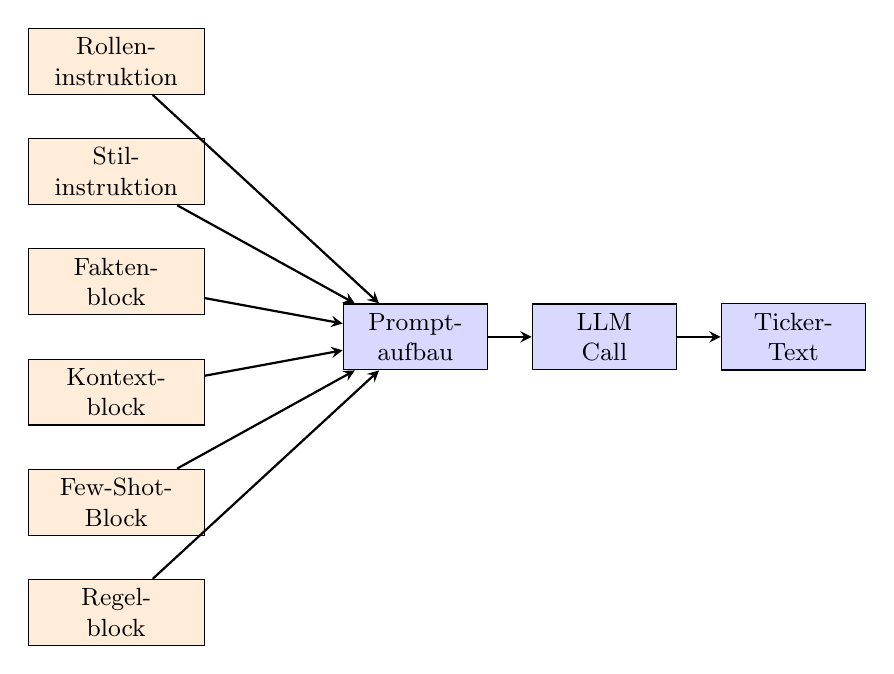
\begin{tikzpicture}
  \tikzset{input/.style={rectangle, draw, fill=orange!15, text width=2.0cm, text centered, minimum height=0.8cm, font=\small}}
  \tikzset{process/.style={rectangle, draw, fill=blue!15, text width=1.6cm, text centered, minimum height=0.8cm, font=\small}}

  % Sechs Bausteine (linke Spalte)
  \node[input] (rolle)    at (0,  0)    {Rollen-\\instruktion};
  \node[input] (stil)     at (0, -1.4)  {Stil-\\instruktion};
  \node[input] (fakten)   at (0, -2.8)  {Fakten-\\block};
  \node[input] (kontext)  at (0, -4.2)  {Kontext-\\block};
  \node[input] (fewshot)  at (0, -5.6)  {Few-Shot-\\Block};
  \node[input] (regeln)   at (0, -7.0)  {Regel-\\block};

  % Verarbeitungsknoten (vertikal zentriert bei -3.5)
  \node[process] (prompt) at (3.8, -3.5) {Prompt-\\aufbau};
  \node[process] (llm)    at (6.2, -3.5) {LLM\\Call};
  \node[process] (output) at (8.6, -3.5) {Ticker-\\Text};

  % Verbindungen
  \draw[arrow] (rolle)   -- (prompt);
  \draw[arrow] (stil)    -- (prompt);
  \draw[arrow] (fakten)  -- (prompt);
  \draw[arrow] (kontext) -- (prompt);
  \draw[arrow] (fewshot) -- (prompt);
  \draw[arrow] (regeln)  -- (prompt);
  \draw[arrow] (prompt)  -- (llm);
  \draw[arrow] (llm)     -- (output);
\end{tikzpicture}%
}


%% DIAGRAM 9: Ticker Generation Flow (Sequence-style, Kapitel 5)
\newcommand{\DiagramTickerGenerationFlow}{%
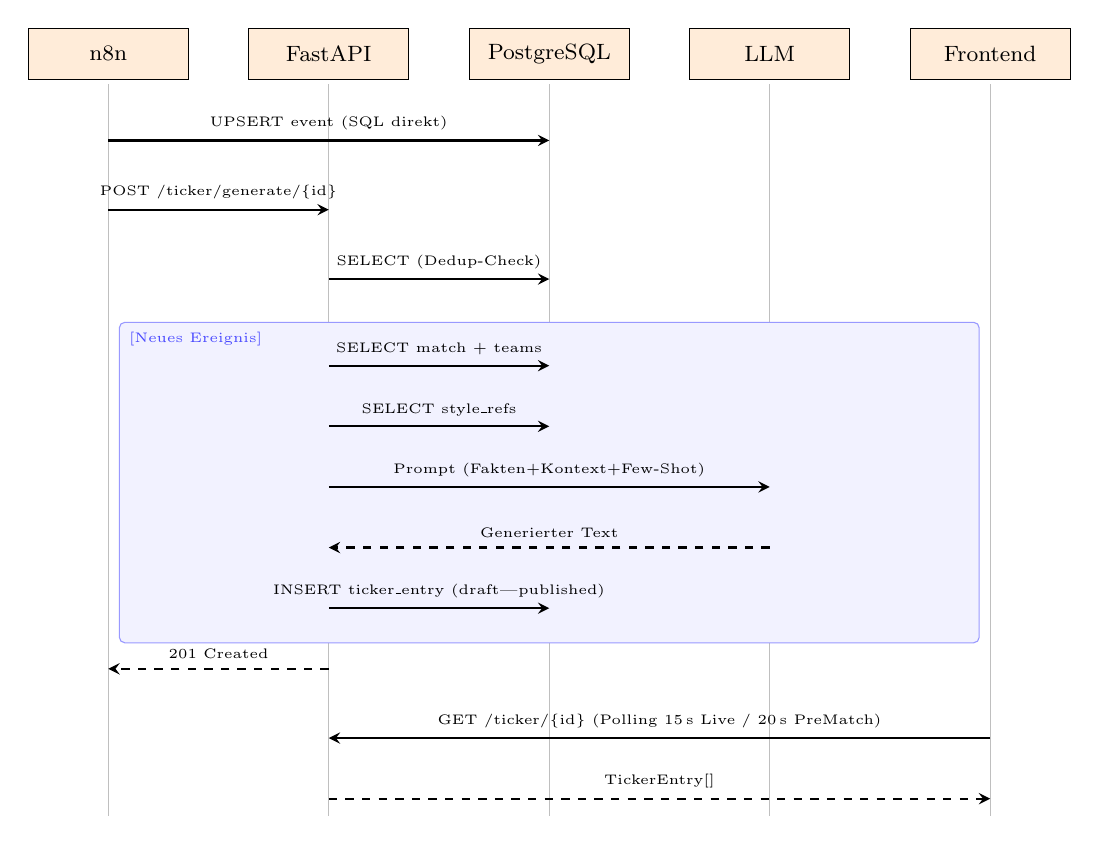
\begin{tikzpicture}[x=2.8cm, y=-1.1cm]
  \tikzset{
    actor/.style={rectangle, draw, fill=orange!15, text width=1.8cm, text centered,
                  minimum height=0.65cm, font=\footnotesize},
    msg/.style={->, thick, >=stealth, font=\tiny},
    retmsg/.style={->, thick, dashed, >=stealth, font=\tiny},
    altbox/.style={draw=blue!40, fill=blue!5, rounded corners=2pt},
  }
  % Participants (top row)
  \foreach \x/\lbl in {0/n8n,1/FastAPI,2/PostgreSQL,3/LLM,4/Frontend}{
    \node[actor] at (\x,0) {\lbl};
    \draw[gray!50, thin] (\x,0.35) -- (\x,8.8);
  }
  % Messages
  \draw[msg]    (0,1)   -- node[above]{UPSERT event (SQL direkt)} (2,1);
  \draw[msg]    (0,1.8) -- node[above]{POST /ticker/generate/\{id\}} (1,1.8);
  \draw[msg]    (1,2.6) -- node[above]{SELECT (Dedup-Check)} (2,2.6);
  % Alt box: Neues Ereignis
  \draw[altbox] (0.05,3.1) rectangle (3.95,6.8);
  \node[font=\tiny, text=blue!70, anchor=north west] at (0.05,3.1) {[Neues Ereignis]};
  \draw[msg]    (1,3.6) -- node[above]{SELECT match + teams} (2,3.6);
  \draw[msg]    (1,4.3) -- node[above]{SELECT style\_refs}   (2,4.3);
  \draw[msg]    (1,5.0) -- node[above]{Prompt (Fakten+Kontext+Few-Shot)} (3,5.0);
  \draw[retmsg] (3,5.7) -- node[above]{Generierter Text}     (1,5.7);
  \draw[msg]    (1,6.4) -- node[above]{INSERT ticker\_entry (draft|published)} (2,6.4);
  \draw[retmsg] (1,7.1) -- node[above]{201 Created}          (0,7.1);
  % Polling
  \draw[msg]    (4,7.9) -- node[above]{GET /ticker/\{id\} (Polling 15\,s Live / 20\,s PreMatch)} (1,7.9);
  \draw[retmsg] (1,8.6) -- node[above]{TickerEntry[]}        (4,8.6);
\end{tikzpicture}%
}


%% ─── DIAGRAM 11: Backend-Schichtenarchitektur ─────────────────────────────
\newcommand{\DiagramBackendSchichten}{%
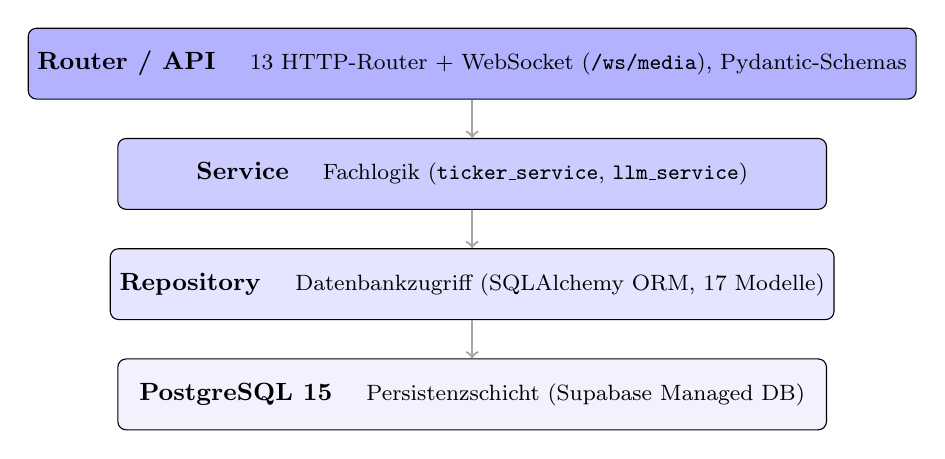
\begin{tikzpicture}[
  layer/.style={draw, rounded corners=3pt,
                minimum width=9cm, minimum height=0.9cm,
                align=center, font=\small},
  arr/.style={->, thick, gray!70}
]
  \node[layer, fill=blue!30] (router) at (0,0)
        {\textbf{Router / API} \quad {\footnotesize 13 HTTP-Router + WebSocket (\texttt{/ws/media}), Pydantic-Schemas}};
  \node[layer, fill=blue!20] (service) at (0,-1.4)
        {\textbf{Service} \quad {\footnotesize Fachlogik (\texttt{ticker\_service}, \texttt{llm\_service})}};
  \node[layer, fill=blue!10] (repo) at (0,-2.8)
        {\textbf{Repository} \quad {\footnotesize Datenbankzugriff (SQLAlchemy ORM, 17 Modelle)}};
  \node[layer, fill=blue!5] (db) at (0,-4.2)
        {\textbf{PostgreSQL 15} \quad {\footnotesize Persistenzschicht (Supabase Managed DB)}};
  \draw[arr] (router) -- (service);
  \draw[arr] (service) -- (repo);
  \draw[arr] (repo) -- (db);
\end{tikzpicture}%
}

%% ─── DIAGRAM 12: Betriebsmodi-Übersicht ──────────────────────────────────
\newcommand{\DiagramBetriebsmodi}{%
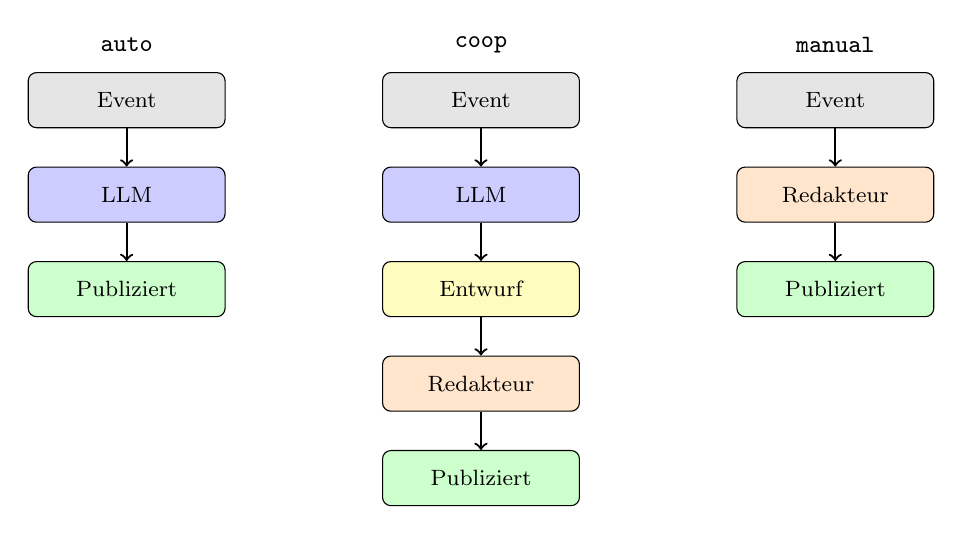
\begin{tikzpicture}[
  box/.style={draw, rounded corners=3pt,
              minimum width=2.5cm, minimum height=0.7cm,
              align=center, font=\footnotesize},
  event/.style={box, fill=gray!20},
  llm/.style={box, fill=blue!20},
  draft/.style={box, fill=yellow!25},
  human/.style={box, fill=orange!20},
  pub/.style={box, fill=green!20},
  arr/.style={->, thick},
  title/.style={font=\small\bfseries}
]
  \node[title]  at (0,   0.7) {\texttt{auto}};
  \node[event]  (ae) at (0,   0)   {Event};
  \node[llm]    (al) at (0,  -1.2) {LLM};
  \node[pub]    (ap) at (0,  -2.4) {Publiziert};
  \draw[arr] (ae)--(al); \draw[arr] (al)--(ap);

  \node[title]  at (4.5, 0.7) {\texttt{coop}};
  \node[event]  (ce) at (4.5,  0)   {Event};
  \node[llm]    (cl) at (4.5, -1.2) {LLM};
  \node[draft]  (cd) at (4.5, -2.4) {Entwurf};
  \node[human]  (cr) at (4.5, -3.6) {Redakteur};
  \node[pub]    (cp) at (4.5, -4.8) {Publiziert};
  \draw[arr] (ce)--(cl); \draw[arr] (cl)--(cd);
  \draw[arr] (cd)--(cr); \draw[arr] (cr)--(cp);

  \node[title]  at (9,   0.7) {\texttt{manual}};
  \node[event]  (me) at (9,   0)   {Event};
  \node[human]  (mr) at (9,  -1.2) {Redakteur};
  \node[pub]    (mp) at (9,  -2.4) {Publiziert};
  \draw[arr] (me)--(mr); \draw[arr] (mr)--(mp);
\end{tikzpicture}%
}

%% ─── DIAGRAM 13: LLM-as-Judge – Qualitätsbewertung nach Stilprofil (pgfplots) ───────────
%% Datenbasis: N=80, Kap6 §6.1.3 (neutral n=27, euphorisch n=27, kritisch n=26)
\newcommand{\DiagramQualitaetStilprofil}{%
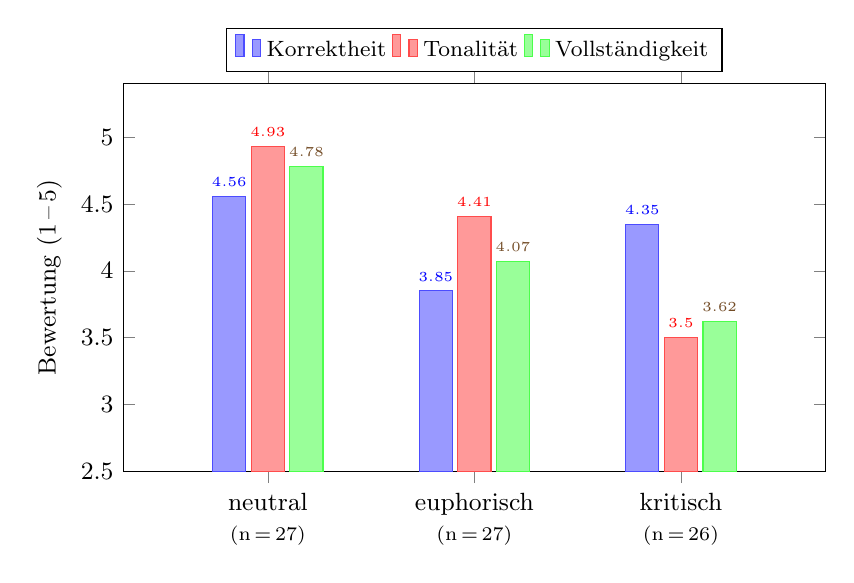
\begin{tikzpicture}
\begin{axis}[
  ybar, bar width=0.42cm,
  width=10.5cm, height=6.5cm,
  ymin=2.5, ymax=5.4,
  ytick={2.5,3.0,3.5,4.0,4.5,5.0},
  ylabel={Bewertung (1\,--\,5)},
  symbolic x coords={neutral, euphorisch, kritisch},
  xtick=data,
  xticklabels={neutral\\{\scriptsize (n\,=\,27)},
               euphorisch\\{\scriptsize (n\,=\,27)},
               kritisch\\{\scriptsize (n\,=\,26)}},
  xticklabel style={align=center},
  legend style={at={(0.5,1.03)}, anchor=south, legend columns=3,
                font=\footnotesize},
  enlarge x limits=0.35,
  nodes near coords,
  nodes near coords style={font=\tiny, /pgf/number format/fixed,
                            /pgf/number format/precision=2},
  every axis/.append style={font=\small},
]
\addplot+[fill=blue!40, draw=blue!70] coordinates {
  (neutral,4.56) (euphorisch,3.85) (kritisch,4.35)
};
\addplot+[fill=red!40, draw=red!70] coordinates {
  (neutral,4.93) (euphorisch,4.41) (kritisch,3.50)
};
\addplot+[fill=green!40, draw=green!70] coordinates {
  (neutral,4.78) (euphorisch,4.07) (kritisch,3.62)
};
\legend{Korrektheit, Tonalit\"at, Vollst\"andigkeit}
\end{axis}
\end{tikzpicture}%
}


%% DIAGRAM: Workflow-Timeline (Spieltag-Gantt)
\newcommand{\DiagramWorkflowTimeline}{%
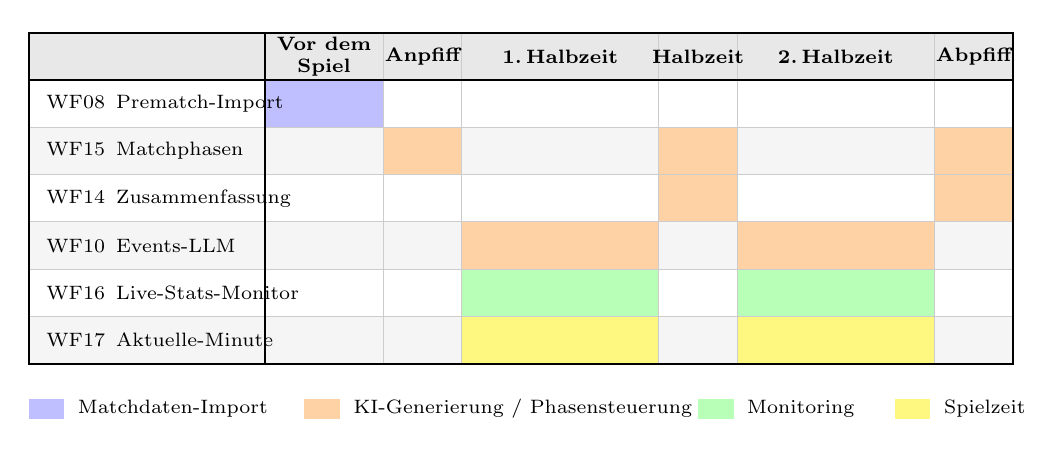
\begin{tikzpicture}[font=\scriptsize]

  % Column left edges (after 3.0 cm label column):
  %  Vor dem Spiel : 3.0–4.5
  %  Anpfiff       : 4.5–5.5
  %  1. Halbzeit   : 5.5–8.0
  %  Halbzeit      : 8.0–9.0
  %  2. Halbzeit   : 9.0–11.5
  %  Abpfiff       :11.5–12.5
  %
  % Row top edges (y, downward):
  %  Header : 0.00 – -0.60
  %  WF08   :-0.60 – -1.20
  %  WF15   :-1.20 – -1.80
  %  WF14   :-1.80 – -2.40
  %  WF10   :-2.40 – -3.00
  %  WF16   :-3.00 – -3.60
  %  WF17   :-3.60 – -4.20

  % Background row fills
  \fill[gray!18] (0,     0   ) rectangle (12.5, -0.60);
  \fill[white]   (0,  -0.60 ) rectangle (12.5, -1.20);
  \fill[gray!8]  (0,  -1.20 ) rectangle (12.5, -1.80);
  \fill[white]   (0,  -1.80 ) rectangle (12.5, -2.40);
  \fill[gray!8]  (0,  -2.40 ) rectangle (12.5, -3.00);
  \fill[white]   (0,  -3.00 ) rectangle (12.5, -3.60);
  \fill[gray!8]  (0,  -3.60 ) rectangle (12.5, -4.20);

  % Active cells
  \fill[blue!25]   ( 3.0, -0.60) rectangle ( 4.5, -1.20); % WF08: Vor dem Spiel
  \fill[orange!35] ( 4.5, -1.20) rectangle ( 5.5, -1.80); % WF15: Anpfiff
  \fill[orange!35] ( 8.0, -1.20) rectangle ( 9.0, -1.80); % WF15: Halbzeit
  \fill[orange!35] (11.5, -1.20) rectangle (12.5, -1.80); % WF15: Abpfiff
  \fill[orange!35] ( 8.0, -1.80) rectangle ( 9.0, -2.40); % WF14: HZ-Zusammenfassung
  \fill[orange!35] (11.5, -1.80) rectangle (12.5, -2.40); % WF14: FT-Zusammenfassung
  \fill[orange!35] ( 5.5, -2.40) rectangle ( 8.0, -3.00); % WF10: 1. Halbzeit
  \fill[orange!35] ( 9.0, -2.40) rectangle (11.5, -3.00); % WF10: 2. Halbzeit
  \fill[green!28]  ( 5.5, -3.00) rectangle ( 8.0, -3.60); % WF16: 1. Halbzeit
  \fill[green!28]  ( 9.0, -3.00) rectangle (11.5, -3.60); % WF16: 2. Halbzeit
  \fill[yellow!50] ( 5.5, -3.60) rectangle ( 8.0, -4.20); % WF17: 1. Halbzeit
  \fill[yellow!50] ( 9.0, -3.60) rectangle (11.5, -4.20); % WF17: 2. Halbzeit

  % Grid lines
  \foreach \y in {0, -0.60, -1.20, -1.80, -2.40, -3.00, -3.60, -4.20} {
    \draw[gray!40, thin] (0, \y) -- (12.5, \y);
  }
  \foreach \x in {0, 3.0, 4.5, 5.5, 8.0, 9.0, 11.5, 12.5} {
    \draw[gray!40, thin] (\x, 0) -- (\x, -4.20);
  }
  \draw[thick] (0, 0) rectangle (12.5, -4.20);
  \draw[thick] (0, -0.60) -- (12.5, -0.60);
  \draw[thick] (3.0, 0) -- (3.0, -4.20);

  % Phase header labels
  \node[font=\scriptsize\bfseries, align=center] at ( 3.75, -0.30) {Vor dem\\Spiel};
  \node[font=\scriptsize\bfseries, align=center] at ( 5.00, -0.30) {Anpfiff};
  \node[font=\scriptsize\bfseries, align=center] at ( 6.75, -0.30) {1.\,Halbzeit};
  \node[font=\scriptsize\bfseries, align=center] at ( 8.50, -0.30) {Halbzeit};
  \node[font=\scriptsize\bfseries, align=center] at (10.25, -0.30) {2.\,Halbzeit};
  \node[font=\scriptsize\bfseries, align=center] at (12.00, -0.30) {Abpfiff};

  % Row labels
  \node[anchor=west] at (0.1, -0.90) {WF08\enspace Prematch-Import};
  \node[anchor=west] at (0.1, -1.50) {WF15\enspace Matchphasen};
  \node[anchor=west] at (0.1, -2.10) {WF14\enspace Zusammenfassung};
  \node[anchor=west] at (0.1, -2.70) {WF10\enspace Events-LLM};
  \node[anchor=west] at (0.1, -3.30) {WF16\enspace Live-Stats-Monitor};
  \node[anchor=west] at (0.1, -3.90) {WF17\enspace Aktuelle-Minute};

  % Legend
  \fill[blue!25]   (0.0, -4.65) rectangle (0.45, -4.90);
  \node[anchor=west] at (0.5,  -4.775) {Matchdaten-Import};
  \fill[orange!35] (3.5, -4.65) rectangle (3.95, -4.90);
  \node[anchor=west] at (4.0,  -4.775) {KI-Generierung / Phasensteuerung};
  \fill[green!28]  (8.5, -4.65) rectangle (8.95, -4.90);
  \node[anchor=west] at (9.0,  -4.775) {Monitoring};
  \fill[yellow!50] (11.0,-4.65) rectangle (11.45,-4.90);
  \node[anchor=west] at (11.5, -4.775) {Spielzeit};

\end{tikzpicture}%
}

%% ────────────────────────────────────────────────────────────────────────────
%% END OF DIAGRAM DEFINITIONS
%% All figures are embedded in their respective chapters using \DiagramXXX commands
%% ────────────────────────────────────────────────────────────────────────────
